\documentclass[a4paper,12pt]{article}
\usepackage{maratona_template}
\usepackage[T1]{fontenc}

\thispagestyle{empty}

\newtheorem{propriedade}{Propriedade}
\newtheorem{definicao}{Definição}

\begin{document}

\begin{center}
\Large{INSTITUTO FEDERAL DO SUL DE MINAS GERIAS}\\
\large{Campus Poços de Caldas}\\
\vspace{10cm}
\Large{Notebook para as Maratonas de Programação}\\
\large{Equipe SK Teletom}
\end{center}

\newpage
\tableofcontents
\thispagestyle{empty}

\newpage
\section{Template}
\inserircodigo{c++}{template.cpp}{8}{8}{}

\newpage
\section{Matemática}
\subsection{Divisão de números inteiros com resto negativo}

Caso seja necessário dividir números inteiros com resto um resto que possivelmente negativo

\inserircodigo{c++}{matematica/div_numeros_inteiros_resto_negativo.cpp}{8}{8}{}

\subsection{Condição existência e classificação de triângulo}

Para um triângulo existir, as três condições devem ser satisfeitas.

\inserircodigo{c++}{matematica/condicao_existencia_triangulo.cpp}{8}{8}{}

\subsection{Comparação entre 2 valores tipo Double}

A comparação entre dois doubles pode retornar valores indejados. Por isso uma função especial para comparação pode ser necessária.

\inserircodigo{c++}{matematica/comparacao_double.cpp}{8}{8}{}

\subsection{Primo rápido – O($\surd$n)}

\inserircodigo{c++}{matematica/primo_rapido_sqrt_n.cpp}{8}{8}{}

\subsection{Crivo de Erastótenes}

\inserircodigo{c++}{matematica/crivo_erastotenes.cpp}{8}{8}{}

\subsection{Checar se um dado bit está ligado}

\inserircodigo{c++}{matematica/check_bit_is_set.cpp}{8}{8}{}

\subsection{Extrair o bit menos significante}

\inserircodigo{c++}{matematica/get_lsb.cpp}{8}{8}{}

\subsection{Contar o número de bits iguais a 1}

\inserircodigo{c++}{matematica/contar_bits_iguais_1.cpp}{8}{8}{}

\subsection{Checar se um número é potência de 2}

\inserircodigo{c++}{matematica/check_is_power_2.cpp}{8}{8}{}

\subsection{Ligar um bit em um número}

\inserircodigo{c++}{matematica/liga_bit_em_numero.cpp}{8}{8}{}

\subsection{Desligar o bit}

\inserircodigo{c++}{matematica/desliga_bit.cpp}{8}{8}{}

\subsection{OR nos Bits ( | )}

\inserircodigo{c++}{matematica/or_nos_bits.cpp}{8}{8}{}

\subsection{AND nos bits (\&)}

\inserircodigo{c++}{matematica/and_nos_bits.cpp}{8}{8}{}

\subsection{XOR nos bits (\textsuperscript{$\wedge$})}

\inserircodigo{c++}{matematica/xor_nos_bits.cpp}{8}{8}{}

\subsection{Shift Esquerdo ( << )}

\inserircodigo{c++}{matematica/shift_esq.cpp}{8}{8}{}

\subsection{Shift Direito ( >> )}

\inserircodigo{c++}{matematica/shift_dir.cpp}{8}{8}{}

\subsection{Arredondamento para cima}

\inserircodigo{c++}{matematica/arrendondamento_cima.cpp}{8}{8}{}

\subsection{Número de casas decimais de um número}

\inserircodigo{c++}{matematica/num_casas_decimais_num.cpp}{8}{8}{}

\subsection{Zerar conteúdo de um array 2d}

\inserircodigo{c++}{matematica/zera_conteudo_array_2d.cpp}{8}{8}{}

\subsection{Zerar conteúdo de um array 1d}

\inserircodigo{c++}{matematica/zera_conteudo_array_1d.cpp}{8}{8}{}

\subsection{Cuidado para divisão de dois floats ou double}

\inserircodigo{c++}{matematica/div_float_double.cpp}{8}{8}{}

\subsection{Conversão inteiro para hexadecimal}

\inserircodigo{c++}{matematica/conversao_int_decimal.cpp}{8}{8}{}

\subsection{Adicionar notação cietífica}

\inserircodigo{c++}{matematica/adc_notacao_cient.cpp}{8}{8}{}

\subsection{Adicionar casas decimais fixas}

\inserircodigo{c++}{matematica/casas_decimais_fixas.cpp}{8}{8}{}

\subsection{Volume do cilindro}

\(pi * r2 * h\)

\subsection{Área Total}

\(A = Ab + Al = 2*\pi*r*(2+h)\) \newline
\(Ab = 2*\pi*r2\) \newline
\(Al = 2*\pi*r*h\)

\subsection{Somatório de Feynman}
Para saber quantos quadrados diferentes existem em um quadriculado de N x N quadrados \newline
\((n*(n+1)*((2*n)+1))/6\)

\subsection{Somatório de um intervalo [a,b] inclusivo}

\(((a + b) * (b - a + 1)) / 2\)

\subsection{Distância entre 2 pontos}

\(sqrt(pow((xf-xi),2) + pow((yf-yi),2))\)

\subsection{Conversão cartesiano para polar}

\( r = \)$\surd$\((a 2 + b2)\)\newline
\(\Phi = tg-1 b/a\)

\subsection{Conversão polar para cartesiano}

\( a = r cos ø\) \newline
\( b = r sem ø\)

\subsection{Número de permutações de um conjunto}

\inserircodigo{c++}{matematica/num_permutacoes_conj.cpp}{8}{8}{}

\subsection{Número de combinações de um conjunto}

\inserircodigo{c++}{matematica/num_combi_conj.cpp}{8}{8}{}

\subsection{Tricks do cmath}

\inserircodigo{c++}{matematica/tricks_cmath.cpp}{8}{8}{}

\subsection{Máximo entre dois números}

\inserircodigo{c++}{matematica/max_entre_dois_num.cpp}{8}{8}{}

\subsection{Mínimo entre dois números}

\inserircodigo{c++}{matematica/min_entre_dois_num.cpp}{8}{8}{}

\subsection{Números primos menores que 100}

// there are 25 numbers\newline
2, 3, 5, 7, 11, 13, 17, 19, 23, 29, 31, 37,\newline
41, 43, 47, 53, 59, 61, 67, 71, 73, 79, 83, 89, 97

\subsection{Maior divisor comum – GCD}

\inserircodigo{c++}{matematica/maior_dc.cpp}{8}{8}{}

\subsection{Menor divisor comum – LCM}

\inserircodigo{c++}{matematica/menor_dc.cpp}{8}{8}{}

\subsection{$A^b$ mod p}

\inserircodigo{c++}{matematica/ab_mod_p.cpp}{8}{8}{}

\subsection{n! mod p}

\inserircodigo{c++}{matematica/n_mod_p.cpp}{8}{8}{}

\subsection{Fatorização de primos}

\inserircodigo{c++}{matematica/fatorizacao_primos.cpp}{8}{8}{}

\newpage
\section{Strings}

\subsection{Modificações}

\subsubsection{Dividir uma string de acordo com um token}

\inserircodigo{c++}{strings/modificacoes/dividir_string_por_token.cpp}{8}{8}{}

\subsubsection{Apagar um intervalo de uma string}

\inserircodigo{c++}{strings/modificacoes/apagar_intervalo_string.cpp}{8}{8}{}

\subsubsection{Remover um caracter de toda a string}

\inserircodigo{c++}{strings/modificacoes/remover_caractere_toda_string.cpp}{8}{8}{}

\subsubsection{Inverter String}

\inserircodigo{c++}{strings/modificacoes/inverter_string.cpp}{8}{8}{}

\subsubsection{Substring}

\inserircodigo{c++}{strings/modificacoes/substring.cpp}{8}{8}{}

\subsection{Verificações}

\subsubsection{Verificar se uma string está vazia}

\inserircodigo{c++}{strings/verificacoes/verifica_string_vazia.cpp}{8}{8}{}

\subsubsection{Verificar se caracter está entre [A-z]}

\inserircodigo{c++}{strings/verificacoes/verifica_caractere_intervalo_A_z.cpp}{8}{8}{}

\subsection{Conversões}

\subsubsection{String para int}

\inserircodigo{c++}{strings/conversoes/string_para_int.cpp}{8}{8}{}

\subsubsection{String para long long}

\inserircodigo{c++}{strings/conversoes/string_para_long_long.cpp}{8}{8}{}

\subsubsection{String para unsigned int}

\inserircodigo{c++}{strings/conversoes/string_para_unsigned_int.cpp}{8}{8}{}

\subsubsection{String para unsigned long long}

\inserircodigo{c++}{strings/conversoes/string_para_unsigned_long_long.cpp}{8}{8}{}

\subsubsection{Char para int}

\inserircodigo{c++}{strings/conversoes/char_para_int.cpp}{8}{8}{}

\subsubsection{Int para String}

\inserircodigo{c++}{strings/conversoes/int_para_string.cpp}{8}{8}{}

\subsubsection{Caracteres minúsculos}

\inserircodigo{c++}{strings/conversoes/caractere_minusculo.cpp}{8}{8}{}

\subsubsection{Caracteres maiúsculos}

\inserircodigo{c++}{strings/conversoes/caractere_maiusculo.cpp}{8}{8}{}

\subsection{Apagar um intervalo de uma string}
\inserircodigo{c++}{strings/modificacoes/apagar_intervalo_string.cpp}{8}{8}{}

\subsection{Remover um caracter de toda a string}
\inserircodigo{c++}{strings/modificacoes/remover_caractere_toda_string.cpp}{8}{8}{}

\subsection{Verificar se uma string está vazia}
\inserircodigo{c++}{strings/verificacoes/verifica_string_vazia.cpp}{8}{8}{}

\subsection{Inverter String}
\inserircodigo{c++}{strings/modificacoes/inverter_string.cpp}{8}{8}{}

\subsection{Criar uma nova string a partir de um intervalo de outra string}
\inserircodigo{c++}{strings/modificacoes/substring.cpp}{8}{8}{}

\subsection{Verificar se caracter está entre [A-z]}
\inserircodigo{c++}{strings/verificacoes/verifica_caractere_intervalo_A_z.cpp}{8}{8}{}

\subsection{Busca [A-z]}
\inserircodigo{c++}{strings/busca.cpp}{8}{8}{}

\subsection{Insert, Erase, Replace}
\inserircodigo{c++}{strings/insert_erase_replace.cpp}{8}{8}{}

\subsection{String Streams}
\inserircodigo{c++}{strings/string_streams.cpp}{8}{8}{}

\newpage
\section{Grafos}
\subsection{Representações de um Grafo}
\subsubsection{Matriz de Adjacência}

\indent\indent A matriz de adjacência consiste em saber, para cada possível par de vértices (u,v), se existe ou não a aresta (u,v).

\indent Vamos guardar na posição (i,j) da matriz a informação sobre a aresta (i,j). Podemos definir 0 para caso ela não existe e 1 para caso ela existe. No caso de termos um grafo com peso, podemos colocar o valor w na posição (i,j), onde w é o peso da aresta (i,j).

\indent Essa representação é fácil de implementar, mas sua complexidade de espaço é muito grande, equivalendo a O(N2), onde N é o número de vértices.

\indent Com relação ao tempo, podemos inserir e deletar uma aresta em O(1), mas saber quais são os vizinhos de um vértice custa O(N).

\indent A representação do grafo fica da seguinte maneira:

\begin{center}
  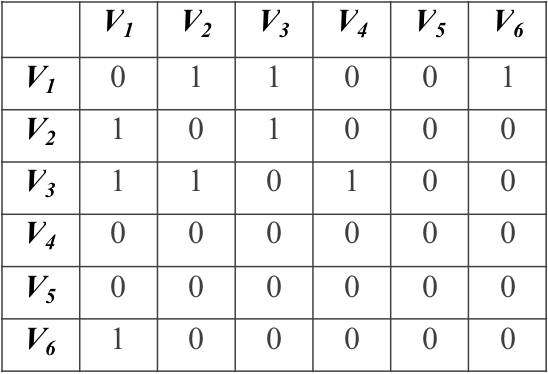
\includegraphics[width=\linewidth/2]{figures/grafos/representacao_matriz_adj.png}
\end{center}

\noindent Implementação em C++:

\inserircodigo{c++}{grafos/matriz_adjacencia.cpp}{8}{8}{}

\subsubsection{Lista de Adjacência}

\indent\indent A lista de adjacência se baseia em guardar, para cada vértice, quais são os seus vizinhos, ou, de uma maneira geral, guardar as arestas que partem desse vértice.

\indent O uso da lista de adjacência pode ser complicado de implementar e debugar para pessoas iniciantes, mas acaba sendo a representação mais usada por pessoas experientes. Isso se deve ao fato de a lista de adjacência possuir complexidade O(1) para inserir novas arestas e um tempo otimizado para consultas num único vértice.

\indent A representação do grafo por lista de adjacência fica da seguinte maneira:

\begin{center}
  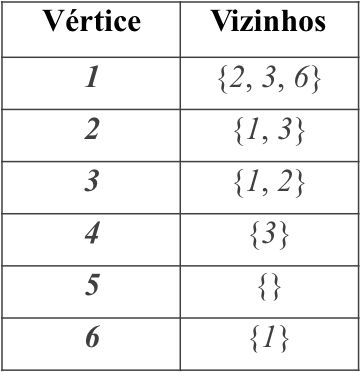
\includegraphics[width=\linewidth/2]{figures/grafos/representacao_lista_adj.png}
\end{center}

\noindent Implementação em C++:

\inserircodigo{c++}{grafos/lista_adjacencia.cpp}{8}{8}{}

\subsection{Lista de Arestas}


\subsection{Algoritmos}
\subsubsection{DFS(Busca em profundidade)}

Como o próprio nome já sugere, o algoritmo começa em um nó raiz e explora tanto quanto possível cada um dos seus ramos, antes de retroceder.

\inserircodigo{c++}{grafos/dfs.cpp}{8}{8}{}

\subsubsection{BFS(Busca em largura)}

\inserircodigo{c++}{grafos/bfs.cpp}{8}{8}{}

\subsubsection{Dijkstra - Caminho Mínimo entre dois pontos}

\inserircodigo{c++}{grafos/dijkstra.cpp}{8}{8}{"Lista de Adjacência"}
\inserircodigo{c++}{grafos/dijkstra_matriz.cpp}{8}{8}{"Matriz de Adjacência"}

\subsubsection{Kruskal - Árvore Geradora Mínima}

Conjunto de arestas com peso mínimo que ligam todo o grafo. \textbf{Para este algoritmo representar grafo utilizando lista de arestas.}

\begin{center}
  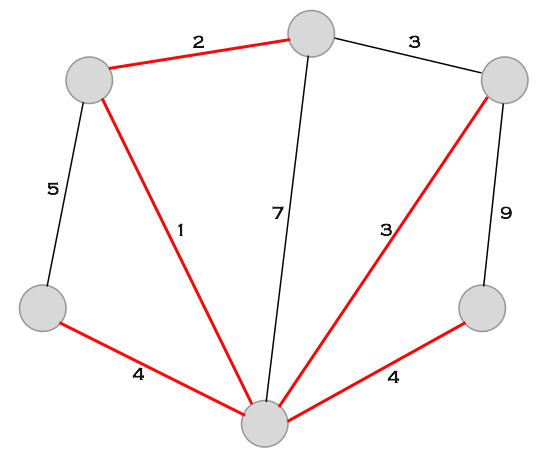
\includegraphics[width=\linewidth/2]{figures/grafos/agm.png}
\end{center}

\subsubsection{Prim - Árvore Geradora Mínima}

Algoritmo parecido com Dijkstra para encontrar árvore geradora mínima.

\noindent Implementação em C++:

\subsubsection{Ordenação Topológica}

\textit{"Malter Warinho está ensinando seu filho a se vestir. Para isso, está dando instruções simples sobre a ordem em que seu filho deve se vestir para não colocar a roupa em ordem contrária (como o Superman). As instruções são do seguinte formato: as meias devem ser colocadas antes do sapatos; as calças devem ser vestidas antes do cinto; a camisa deve ser vestida antes do casaco; e por aí vai. Em alguns casos, não interessa a ordem em que deve ser colocada a roupa. Por exemplo, o filho pode colocar as calças antes do chapéu e vice-versa. Dada a lista de instruções e o número de peças de roupas, ajude o filho de Malter a se vestir."}\newline

\noindent Bem, para formalizar um pouco o problema, vamos montar um grafo direcionado onde:

\begin{itemize}
    \item cada vértice é uma peça de roupa.
    \item cada aresta partindo de um vértice X para um vértice Y significa que X tem que vir antes de Y.
\end{itemize}

\noindent Assim, pode se notar uma relação de transição: se X tem que vir antes de Y e Y tem que vir antes de Z, X tem que vir antes de Z.

\noindent Teremos então um grafo semelhante a este:

\begin{center}
  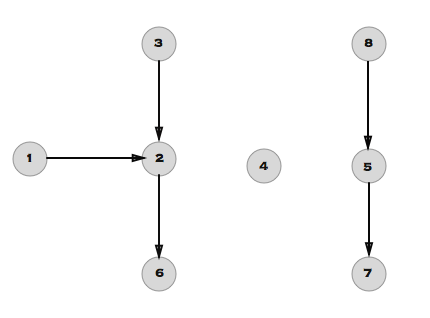
\includegraphics[width=\linewidth/2]{figures/grafos/OT.png}
\end{center}

\noindent Tendo uma noção do grafo, é fácil perceber alguns fatos simples:

\begin{itemize}
    \item se o grafo possui um ciclo, não há ordem em que se possa resolver o problema.
    \item podemos executar um vértice (vestir uma roupa) se, e somente se, todos os vértices (roupas) que possuem algum caminho até ele já foram executados.
\end{itemize}

\noindent Com apenas isso, já se pode pensar em um algoritmo bem simples para resolver o problema:

\begin{itemize}
    \item Pegar um vértice de grau de entrada zero (nenhuma aresta chega a ele) e acrescentar o vértice a ordem de execução.
    \item Remover todas as arestas que partem desse vértice e atualizar os graus dos vértices ligados a essas arestas.
    \item Repetir o processo até não haver mais vértices de grau de entrada zero (ou acabarem todos os vértices).
\end{itemize}

\noindent Se, ao final do processo, ainda sobrarem vértices, há um ciclo e não há ordem para resolver o problema. Caso contrário, o problema está resolvido.

\noindent Implementação em C++:

\subsubsection{Floyd-Warshall - Menor Caminho}

Menor distância de qualquer vértice para qualquer outro.

\subsubsection{LCA - Menor Ancestral Comum}

Ancestral comum mais próximo à dois vértices.

\begin{center}
  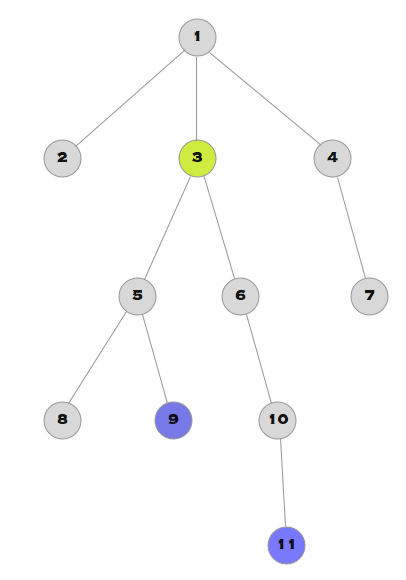
\includegraphics[width=\linewidth/2]{figures/grafos/LCA.png}
\end{center}

\subsubsection{Caminho Euleriano}

Um Caminho Euleriano de um grafo é um trajeto que passa por todas as arestas do grafo sem repetição.

\noindent\textbf{Existência:} Porém, antes de procurarmos um Caminho Euleriano para um grafo, precisamos saber se ele existe. Checar a existência de um Caminho Euleriano é, na verdade, bem fácil. Para um grafo ter um Caminho Euleriano, é suficiente e necessário satisfazer uma de duas condições:
\begin{itemize}
    \item Todos os vértices do grafo tem que ter grau par.
    \item Todos os vértices (ignorando-se os de grau zero) tem grau par, exceto dois vértices que possuem grau ímpar. Nesse caso, os dois vértices de grau ímpar são o início e o fim do Caminho.
\end{itemize}

\noindent Implementação em C++:

\subsubsection{Grafos bipartidos}
Um grafo é dito bipartido quando seus vértices podem ser divididos em dois conjuntos disjuntos tais que cada aresta ligue apenas vértices de grupos diferente.

\begin{center}
  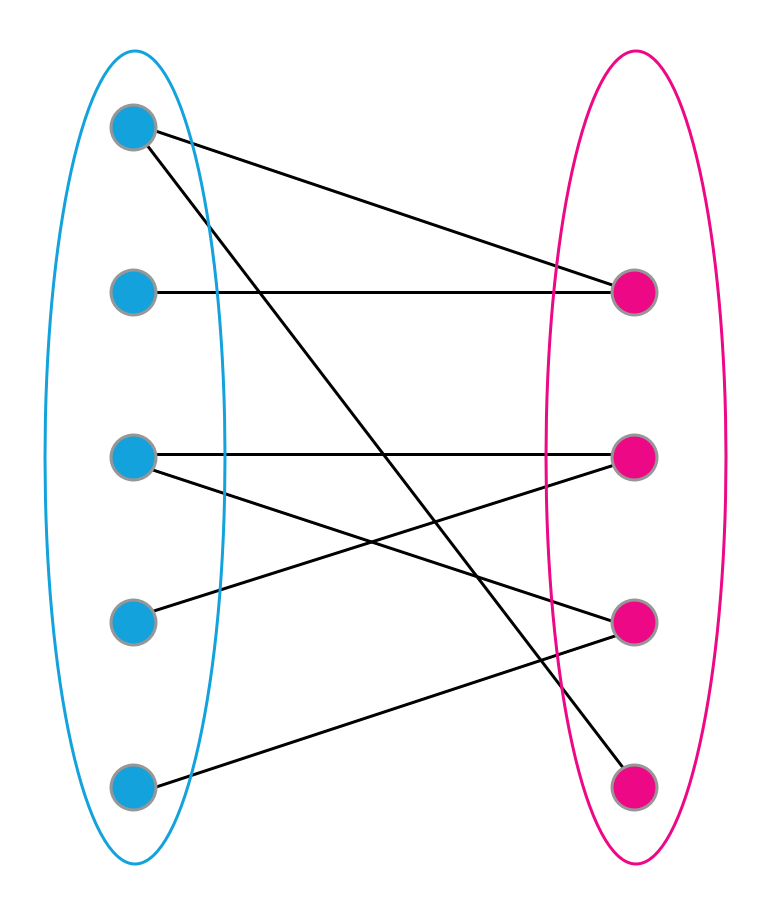
\includegraphics[width=\linewidth/2]{figures/grafos/grafos_bipartidos.png}
\end{center}

\noindent Implementação em C++:

\newpage

\section{Programação dinâmica}

\indent Aplicar a programação dinâmica se:

\begin{itemize}
    \item É possível dividir o problema em problemas menores.
    \item É possível encontrar as soluções ótimas para os subproblemas.
    \item Há sobreposição de subproblemas, isto é, há subproblemas que compartilham as mesmas respostas ótimas.
\end{itemize}

\subsection{Problema da mochila}

\indent O problema da mochila consiste de uma mochila de capacidade total $C$ e de $N$ itens que podem ser colocados dentro da mochila. Cada item possui um peso $p_i$ e um valor $v_i$. Objetiva-se colocar o maior número de itens dentro da mochila a fim de maximizar o valor total dos itens colocados. Matematicamente:

\begin{equation}
    \max \sum\limits_{i=1}^{I}v_i,
\end{equation}

\noindent onde $I$ é o conjunto de itens dentro da mochila. Sujeito as restrições:

\begin{equation}
    \sum\limits_{i=1}^{I}p_i \leq C
\end{equation}
\inserircodigo{c}{programacao_dinamica/mochila.c}{8}{8}{}

\subsection{Problema do troco}

\subsection{Problema do corte de hastes}

Dada uma haste de tamanho $n$ e o preço $p_i$ do corte de tamanho $i$. Qual é a melhor maneira de cortar a haste para maximizar o preço?

\inserircodigo{c}{programacao_dinamica/corte_haste.c}{8}{8}{}

\end{document}